% Options for packages loaded elsewhere
\PassOptionsToPackage{unicode}{hyperref}
\PassOptionsToPackage{hyphens}{url}
%
\documentclass[
]{article}
\usepackage{amsmath,amssymb}
\usepackage{lmodern}
\usepackage{iftex}
\ifPDFTeX
  \usepackage[T1]{fontenc}
  \usepackage[utf8]{inputenc}
  \usepackage{textcomp} % provide euro and other symbols
\else % if luatex or xetex
  \usepackage{unicode-math}
  \defaultfontfeatures{Scale=MatchLowercase}
  \defaultfontfeatures[\rmfamily]{Ligatures=TeX,Scale=1}
\fi
% Use upquote if available, for straight quotes in verbatim environments
\IfFileExists{upquote.sty}{\usepackage{upquote}}{}
\IfFileExists{microtype.sty}{% use microtype if available
  \usepackage[]{microtype}
  \UseMicrotypeSet[protrusion]{basicmath} % disable protrusion for tt fonts
}{}
\makeatletter
\@ifundefined{KOMAClassName}{% if non-KOMA class
  \IfFileExists{parskip.sty}{%
    \usepackage{parskip}
  }{% else
    \setlength{\parindent}{0pt}
    \setlength{\parskip}{6pt plus 2pt minus 1pt}}
}{% if KOMA class
  \KOMAoptions{parskip=half}}
\makeatother
\usepackage{xcolor}
\usepackage[margin=1in]{geometry}
\usepackage{color}
\usepackage{fancyvrb}
\newcommand{\VerbBar}{|}
\newcommand{\VERB}{\Verb[commandchars=\\\{\}]}
\DefineVerbatimEnvironment{Highlighting}{Verbatim}{commandchars=\\\{\}}
% Add ',fontsize=\small' for more characters per line
\usepackage{framed}
\definecolor{shadecolor}{RGB}{248,248,248}
\newenvironment{Shaded}{\begin{snugshade}}{\end{snugshade}}
\newcommand{\AlertTok}[1]{\textcolor[rgb]{0.94,0.16,0.16}{#1}}
\newcommand{\AnnotationTok}[1]{\textcolor[rgb]{0.56,0.35,0.01}{\textbf{\textit{#1}}}}
\newcommand{\AttributeTok}[1]{\textcolor[rgb]{0.77,0.63,0.00}{#1}}
\newcommand{\BaseNTok}[1]{\textcolor[rgb]{0.00,0.00,0.81}{#1}}
\newcommand{\BuiltInTok}[1]{#1}
\newcommand{\CharTok}[1]{\textcolor[rgb]{0.31,0.60,0.02}{#1}}
\newcommand{\CommentTok}[1]{\textcolor[rgb]{0.56,0.35,0.01}{\textit{#1}}}
\newcommand{\CommentVarTok}[1]{\textcolor[rgb]{0.56,0.35,0.01}{\textbf{\textit{#1}}}}
\newcommand{\ConstantTok}[1]{\textcolor[rgb]{0.00,0.00,0.00}{#1}}
\newcommand{\ControlFlowTok}[1]{\textcolor[rgb]{0.13,0.29,0.53}{\textbf{#1}}}
\newcommand{\DataTypeTok}[1]{\textcolor[rgb]{0.13,0.29,0.53}{#1}}
\newcommand{\DecValTok}[1]{\textcolor[rgb]{0.00,0.00,0.81}{#1}}
\newcommand{\DocumentationTok}[1]{\textcolor[rgb]{0.56,0.35,0.01}{\textbf{\textit{#1}}}}
\newcommand{\ErrorTok}[1]{\textcolor[rgb]{0.64,0.00,0.00}{\textbf{#1}}}
\newcommand{\ExtensionTok}[1]{#1}
\newcommand{\FloatTok}[1]{\textcolor[rgb]{0.00,0.00,0.81}{#1}}
\newcommand{\FunctionTok}[1]{\textcolor[rgb]{0.00,0.00,0.00}{#1}}
\newcommand{\ImportTok}[1]{#1}
\newcommand{\InformationTok}[1]{\textcolor[rgb]{0.56,0.35,0.01}{\textbf{\textit{#1}}}}
\newcommand{\KeywordTok}[1]{\textcolor[rgb]{0.13,0.29,0.53}{\textbf{#1}}}
\newcommand{\NormalTok}[1]{#1}
\newcommand{\OperatorTok}[1]{\textcolor[rgb]{0.81,0.36,0.00}{\textbf{#1}}}
\newcommand{\OtherTok}[1]{\textcolor[rgb]{0.56,0.35,0.01}{#1}}
\newcommand{\PreprocessorTok}[1]{\textcolor[rgb]{0.56,0.35,0.01}{\textit{#1}}}
\newcommand{\RegionMarkerTok}[1]{#1}
\newcommand{\SpecialCharTok}[1]{\textcolor[rgb]{0.00,0.00,0.00}{#1}}
\newcommand{\SpecialStringTok}[1]{\textcolor[rgb]{0.31,0.60,0.02}{#1}}
\newcommand{\StringTok}[1]{\textcolor[rgb]{0.31,0.60,0.02}{#1}}
\newcommand{\VariableTok}[1]{\textcolor[rgb]{0.00,0.00,0.00}{#1}}
\newcommand{\VerbatimStringTok}[1]{\textcolor[rgb]{0.31,0.60,0.02}{#1}}
\newcommand{\WarningTok}[1]{\textcolor[rgb]{0.56,0.35,0.01}{\textbf{\textit{#1}}}}
\usepackage{longtable,booktabs,array}
\usepackage{calc} % for calculating minipage widths
% Correct order of tables after \paragraph or \subparagraph
\usepackage{etoolbox}
\makeatletter
\patchcmd\longtable{\par}{\if@noskipsec\mbox{}\fi\par}{}{}
\makeatother
% Allow footnotes in longtable head/foot
\IfFileExists{footnotehyper.sty}{\usepackage{footnotehyper}}{\usepackage{footnote}}
\makesavenoteenv{longtable}
\usepackage{graphicx}
\makeatletter
\def\maxwidth{\ifdim\Gin@nat@width>\linewidth\linewidth\else\Gin@nat@width\fi}
\def\maxheight{\ifdim\Gin@nat@height>\textheight\textheight\else\Gin@nat@height\fi}
\makeatother
% Scale images if necessary, so that they will not overflow the page
% margins by default, and it is still possible to overwrite the defaults
% using explicit options in \includegraphics[width, height, ...]{}
\setkeys{Gin}{width=\maxwidth,height=\maxheight,keepaspectratio}
% Set default figure placement to htbp
\makeatletter
\def\fps@figure{htbp}
\makeatother
\setlength{\emergencystretch}{3em} % prevent overfull lines
\providecommand{\tightlist}{%
  \setlength{\itemsep}{0pt}\setlength{\parskip}{0pt}}
\setcounter{secnumdepth}{-\maxdimen} % remove section numbering
\ifLuaTeX
  \usepackage{selnolig}  % disable illegal ligatures
\fi
\IfFileExists{bookmark.sty}{\usepackage{bookmark}}{\usepackage{hyperref}}
\IfFileExists{xurl.sty}{\usepackage{xurl}}{} % add URL line breaks if available
\urlstyle{same} % disable monospaced font for URLs
\hypersetup{
  pdftitle={Chapter 13: General Linear Models},
  pdfauthor={Ram Gopal, Dan Philps, and Tillman Weyde},
  hidelinks,
  pdfcreator={LaTeX via pandoc}}

\title{Chapter 13: General Linear Models}
\author{Ram Gopal, Dan Philps, and Tillman Weyde}
\date{Summer 20202}

\begin{document}
\maketitle

{
\setcounter{tocdepth}{4}
\tableofcontents
}
\hypertarget{load-packages}{%
\section{Load packages}\label{load-packages}}

\begin{Shaded}
\begin{Highlighting}[]
\FunctionTok{library}\NormalTok{(bbmle)}
\FunctionTok{set.seed}\NormalTok{(}\DecValTok{987654321}\NormalTok{)}
\end{Highlighting}
\end{Shaded}

\hypertarget{binary-outcomes}{%
\section{Binary Outcomes}\label{binary-outcomes}}

\hypertarget{baseline-model}{%
\subsection{Baseline Model}\label{baseline-model}}

The baseline model that we want to estimate is shown in the following
figure.

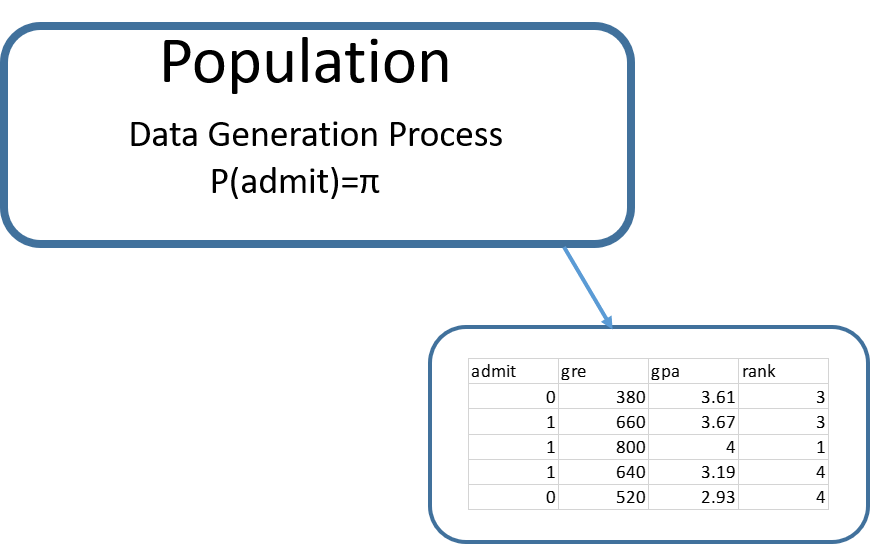
\includegraphics{estpic11.png}

\begin{Shaded}
\begin{Highlighting}[]
\NormalTok{admit }\OtherTok{\textless{}{-}} \FunctionTok{read.csv}\NormalTok{(}\StringTok{"../../data/admit.csv"}\NormalTok{)}
\NormalTok{LLbinary }\OtherTok{=} \ControlFlowTok{function}\NormalTok{(pi)\{}
\NormalTok{  p }\OtherTok{=} \FunctionTok{ifelse}\NormalTok{(admit}\SpecialCharTok{$}\NormalTok{admit }\SpecialCharTok{==} \DecValTok{1}\NormalTok{, pi, }\DecValTok{1} \SpecialCharTok{{-}}\NormalTok{ pi)}
\NormalTok{  LL }\OtherTok{=} \FunctionTok{sum}\NormalTok{(}\FunctionTok{log}\NormalTok{(p))}
  \FunctionTok{return}\NormalTok{(}\SpecialCharTok{{-}}\DecValTok{1}\SpecialCharTok{*}\NormalTok{LL)}
\NormalTok{\}}

\NormalTok{res1 }\OtherTok{=} \FunctionTok{mle2}\NormalTok{(}\AttributeTok{minuslogl =}\NormalTok{ LLbinary, }\AttributeTok{start =} \FunctionTok{list}\NormalTok{(}\AttributeTok{pi=}\NormalTok{ .}\DecValTok{5}\NormalTok{))}
\FunctionTok{summary}\NormalTok{(res1)}
\end{Highlighting}
\end{Shaded}

\begin{verbatim}
## Maximum likelihood estimation
## 
## Call:
## mle2(minuslogl = LLbinary, start = list(pi = 0.5))
## 
## Coefficients:
##    Estimate Std. Error z value               Pr(z)    
## pi   0.3175     0.0233    13.6 <0.0000000000000002 ***
## ---
## Signif. codes:  0 '***' 0.001 '**' 0.01 '*' 0.05 '.' 0.1 ' ' 1
## 
## -2 log L: 500
\end{verbatim}

Now suppose we think that the probability of admission is determined by
the variables gre, gpa, and rank. The data generation process is
depicted in the following figure.

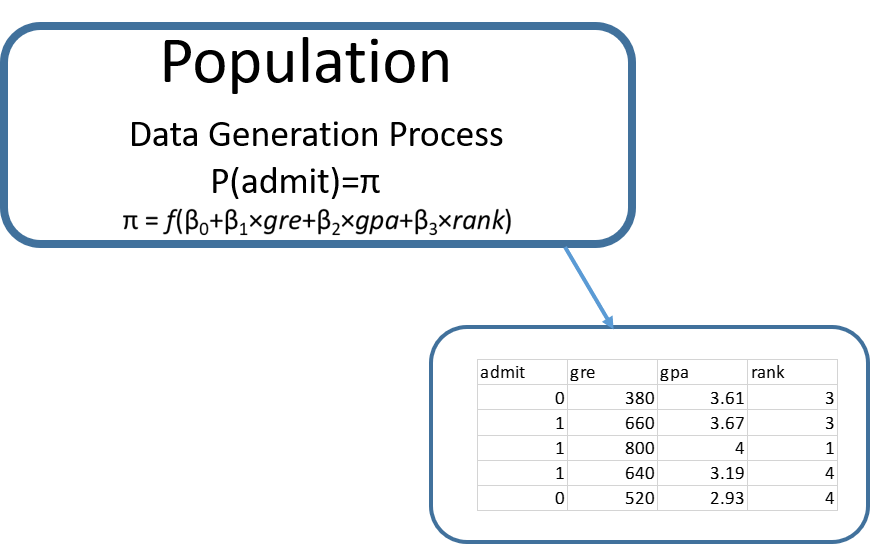
\includegraphics{estpic12.png}

Let us denote

\[X = \beta_0 + \beta_1 \times gre + \beta_2 \times gpa + \beta_3 \times rank\]

What should the function be that links X with \(\pi\)? The issue here is
that the two terms have different domains. The domain for \(\pi\) is
\([0,1]\). The domain for X on the other hand is \((-\infty,\infty)\).
For the function \(f\) that relates X to \(\pi\), we need to be able to
match the two domains. The function \(f\) is called the \textbf{link}
function.

\hypertarget{logistic-regression}{%
\subsection{Logistic Regression}\label{logistic-regression}}

The following table illustrates the creation of one possible link
function.

\begin{longtable}[]{@{}ll@{}}
\toprule()
Variable & Domain \\
\midrule()
\endhead
X & \([-\infty,\infty]\) \\
\(e^X\) & \([0,\infty]\) \\
\(\frac{e^X}{1 + e^X}\) & {[}0,1{]} \\
\bottomrule()
\end{longtable}

\begin{center}\rule{0.5\linewidth}{0.5pt}\end{center}

The specification linking \(\pi\) with X is the following.

\[\pi = \frac{e^X}{1 + e^X}\]

Rearranging this gives us what is called the \textbf{logistic regression
specification}.

\[ln(\frac{\pi}{1-\pi}) = X = \beta_0 + \beta_1 \times gre + \beta_2 \times gpa + \beta_3 \times rank\]

In terms of the terminology, \(\pi\) is the probability of
\textbf{success}, \(\frac{\pi}{1-\pi}\) is called the \textbf{odds}, and
\(log(\frac{\pi}{1-\pi})\) is the \textbf{log-odds}. The logistic
regression specification essentially says that the log-odds are a linear
function of the independent variables.

Now, let us write the code to estimate this.

\begin{Shaded}
\begin{Highlighting}[]
\NormalTok{LLbinary }\OtherTok{=} \ControlFlowTok{function}\NormalTok{(b0,b1,b2,b3)\{}
\NormalTok{    X }\OtherTok{=}\NormalTok{ b0 }\SpecialCharTok{+}\NormalTok{ b1}\SpecialCharTok{*}\NormalTok{admit}\SpecialCharTok{$}\NormalTok{gre }\SpecialCharTok{+}\NormalTok{ b2}\SpecialCharTok{*}\NormalTok{admit}\SpecialCharTok{$}\NormalTok{gpa }\SpecialCharTok{+}\NormalTok{ b3}\SpecialCharTok{*}\NormalTok{admit}\SpecialCharTok{$}\NormalTok{rank}
\NormalTok{    pi }\OtherTok{=} \FunctionTok{exp}\NormalTok{(X)}\SpecialCharTok{/}\NormalTok{(}\DecValTok{1}\SpecialCharTok{+}\NormalTok{(}\FunctionTok{exp}\NormalTok{(X)))}
\NormalTok{    p }\OtherTok{=} \FunctionTok{ifelse}\NormalTok{(admit}\SpecialCharTok{$}\NormalTok{admit }\SpecialCharTok{==} \DecValTok{1}\NormalTok{, pi, }\DecValTok{1} \SpecialCharTok{{-}}\NormalTok{ pi)}
\NormalTok{  LL }\OtherTok{=} \FunctionTok{sum}\NormalTok{(}\FunctionTok{log}\NormalTok{(p))}
  \FunctionTok{return}\NormalTok{(}\SpecialCharTok{{-}}\DecValTok{1}\SpecialCharTok{*}\NormalTok{LL)}
\NormalTok{\}}

\NormalTok{res2 }\OtherTok{=} \FunctionTok{mle2}\NormalTok{(}\AttributeTok{minuslogl =}\NormalTok{ LLbinary, }\AttributeTok{start =} \FunctionTok{list}\NormalTok{(}\AttributeTok{b0 =} \DecValTok{0}\NormalTok{, }\AttributeTok{b1 =} \DecValTok{0}\NormalTok{, }\AttributeTok{b2 =} \DecValTok{0}\NormalTok{, }\AttributeTok{b3 =} \DecValTok{0}\NormalTok{))}
\FunctionTok{summary}\NormalTok{(res2)}
\end{Highlighting}
\end{Shaded}

\begin{verbatim}
## Maximum likelihood estimation
## 
## Call:
## mle2(minuslogl = LLbinary, start = list(b0 = 0, b1 = 0, b2 = 0, 
##     b3 = 0))
## 
## Coefficients:
##    Estimate Std. Error z value     Pr(z)    
## b0 -3.34596    1.13080   -2.96    0.0031 ** 
## b1  0.00169    0.00109    1.55    0.1204    
## b2  0.88048    0.32901    2.68    0.0074 ** 
## b3 -0.59679    0.12797   -4.66 0.0000031 ***
## ---
## Signif. codes:  0 '***' 0.001 '**' 0.01 '*' 0.05 '.' 0.1 ' ' 1
## 
## -2 log L: 459.8
\end{verbatim}

The estimated logistic regression is the following.

\[ln(\frac{\pi}{1-\pi}) = -3.35 + 0.0017 \times gre + 0.88 \times gpa - 0.60 \times rank\]

The results indicate that gre is not statistically significant. A higher
gpa increases the log-odds of admission, and higher rank lowers the
log-odds of admission.

Let us try to understand the marginal effects. A unit increase in gpa
increases the log-odds by 0.88. To understand this further, we can write

\[ln(\frac{\pi_1}{1-\pi_1}) - ln(\frac{\pi}{1-\pi}) = .88\]

Rearranging this, we get

\[\frac{\pi_1}{1-\pi_1}= \frac{\pi}{1-\pi}e^{0.88}\]

\[\frac{\pi_1}{1-\pi_1}= 2.41\frac{\pi}{1-\pi}\]

Thus, we can say that a unit increase in gpa increases the odds of
admission by a factor of 2.41.

\hypertarget{probit-regression}{%
\subsection{Probit Regression}\label{probit-regression}}

Another way to create the link function between X and \(\pi\) is to use
the following.

\[\pi = \Phi (X)\]

where \(\Phi(X)\) is a cumulative probability of a standard normal
distribution. This is called a probit regression. Let us code this.

\begin{Shaded}
\begin{Highlighting}[]
\NormalTok{LLbinary }\OtherTok{=} \ControlFlowTok{function}\NormalTok{(b0,b1,b2,b3)\{}
\NormalTok{    X }\OtherTok{=}\NormalTok{ b0 }\SpecialCharTok{+}\NormalTok{ b1}\SpecialCharTok{*}\NormalTok{admit}\SpecialCharTok{$}\NormalTok{gre }\SpecialCharTok{+}\NormalTok{ b2}\SpecialCharTok{*}\NormalTok{admit}\SpecialCharTok{$}\NormalTok{gpa }\SpecialCharTok{+}\NormalTok{ b3}\SpecialCharTok{*}\NormalTok{admit}\SpecialCharTok{$}\NormalTok{rank}
\NormalTok{    pi }\OtherTok{=} \FunctionTok{pnorm}\NormalTok{(X)}
\NormalTok{    p }\OtherTok{=} \FunctionTok{ifelse}\NormalTok{(admit}\SpecialCharTok{$}\NormalTok{admit }\SpecialCharTok{==} \DecValTok{1}\NormalTok{, pi, }\DecValTok{1} \SpecialCharTok{{-}}\NormalTok{ pi)}
\NormalTok{  LL }\OtherTok{=} \FunctionTok{sum}\NormalTok{(}\FunctionTok{log}\NormalTok{(p))}
  \FunctionTok{return}\NormalTok{(}\SpecialCharTok{{-}}\DecValTok{1}\SpecialCharTok{*}\NormalTok{LL)}
\NormalTok{\}}

\NormalTok{res3 }\OtherTok{=} \FunctionTok{mle2}\NormalTok{(}\AttributeTok{minuslogl =}\NormalTok{ LLbinary, }\AttributeTok{start =} \FunctionTok{list}\NormalTok{(}\AttributeTok{b0 =} \DecValTok{0}\NormalTok{, }\AttributeTok{b1 =} \DecValTok{0}\NormalTok{, }\AttributeTok{b2 =} \DecValTok{0}\NormalTok{, }\AttributeTok{b3 =} \DecValTok{0}\NormalTok{))}
\FunctionTok{summary}\NormalTok{(res3)}
\end{Highlighting}
\end{Shaded}

\begin{verbatim}
## Maximum likelihood estimation
## 
## Call:
## mle2(minuslogl = LLbinary, start = list(b0 = 0, b1 = 0, b2 = 0, 
##     b3 = 0))
## 
## Coefficients:
##     Estimate Std. Error z value     Pr(z)    
## b0 -2.084272   0.671707   -3.10    0.0019 ** 
## b1  0.000930   0.000645    1.44    0.1494    
## b2  0.558801   0.194190    2.88    0.0040 ** 
## b3 -0.352533   0.074458   -4.73 0.0000022 ***
## ---
## Signif. codes:  0 '***' 0.001 '**' 0.01 '*' 0.05 '.' 0.1 ' ' 1
## 
## -2 log L: 460.1
\end{verbatim}

You will see that the results are pretty similar to the logistic
regression. The coefficients in a probit regression are a bit harder to
interpret, and therefore the logistic regression is more commonly used.

\hypertarget{count-outcomes}{%
\section{Count Outcomes}\label{count-outcomes}}

Let us read the file \texttt{student.csv}.

\begin{Shaded}
\begin{Highlighting}[]
\NormalTok{student }\OtherTok{\textless{}{-}} \FunctionTok{read.csv}\NormalTok{(}\StringTok{"../../data/student.csv"}\NormalTok{)}
\FunctionTok{head}\NormalTok{(student)}
\end{Highlighting}
\end{Shaded}

\begin{verbatim}
##     id gender math prog daysabs
## 1 1001      0   63    2       4
## 2 1002      0   27    2       4
## 3 1003      1   20    2       2
## 4 1004      1   16    2       3
## 5 1005      1    2    2       3
## 6 1006      1   71    2      13
\end{verbatim}

\hypertarget{baseline-model-1}{%
\subsection{Baseline Model}\label{baseline-model-1}}

The outcome of interest is the variable daysabs, the number of days a
student was absent. The baseline model is depicted below.
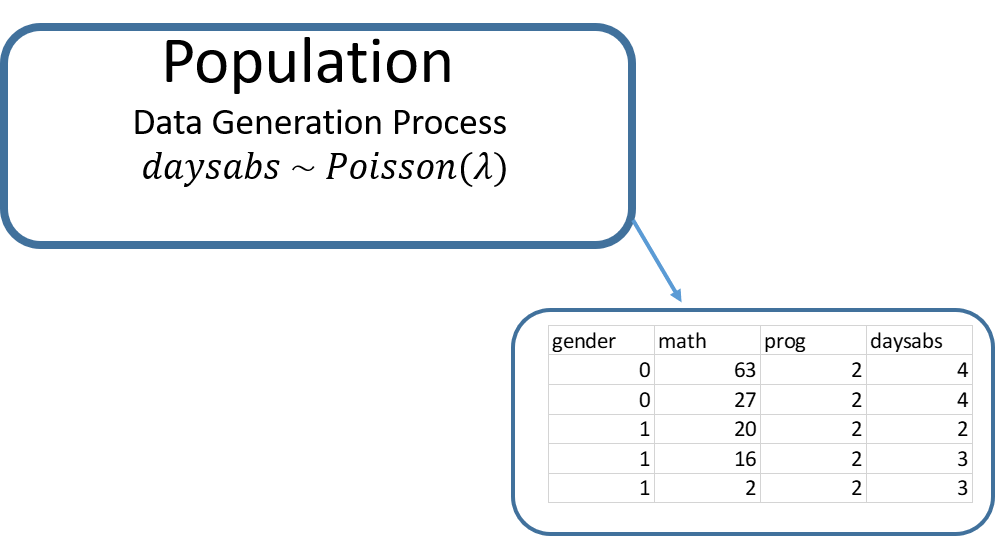
\includegraphics{estpic13.png}

The following estimates the population parameter \(\lambda\).

\begin{Shaded}
\begin{Highlighting}[]
\NormalTok{LLpois }\OtherTok{=} \ControlFlowTok{function}\NormalTok{(lam)\{}
\NormalTok{  p }\OtherTok{=} \FunctionTok{dpois}\NormalTok{(}\AttributeTok{x =}\NormalTok{ student}\SpecialCharTok{$}\NormalTok{daysabs, }\AttributeTok{lambda =}\NormalTok{ lam)}
\NormalTok{  LL }\OtherTok{=} \FunctionTok{sum}\NormalTok{(}\FunctionTok{log}\NormalTok{(p))}
  \FunctionTok{return}\NormalTok{(}\SpecialCharTok{{-}}\DecValTok{1}\SpecialCharTok{*}\NormalTok{LL)}
\NormalTok{\}}

\NormalTok{res4 }\OtherTok{=} \FunctionTok{mle2}\NormalTok{(}\AttributeTok{minuslogl =}\NormalTok{ LLpois, }\AttributeTok{start =} \FunctionTok{list}\NormalTok{(}\AttributeTok{lam=}\DecValTok{10}\NormalTok{))}
\FunctionTok{summary}\NormalTok{(res4)}
\end{Highlighting}
\end{Shaded}

\begin{verbatim}
## Maximum likelihood estimation
## 
## Call:
## mle2(minuslogl = LLpois, start = list(lam = 10))
## 
## Coefficients:
##     Estimate Std. Error z value               Pr(z)    
## lam    5.955      0.138    43.2 <0.0000000000000002 ***
## ---
## Signif. codes:  0 '***' 0.001 '**' 0.01 '*' 0.05 '.' 0.1 ' ' 1
## 
## -2 log L: 3101
\end{verbatim}

\hypertarget{poisson-regression}{%
\subsection{Poisson Regression}\label{poisson-regression}}

Now suppose we think that the number of days absent is influenced by the
variables gender, math, and prog. The data generation process is
depicted in the following figure.

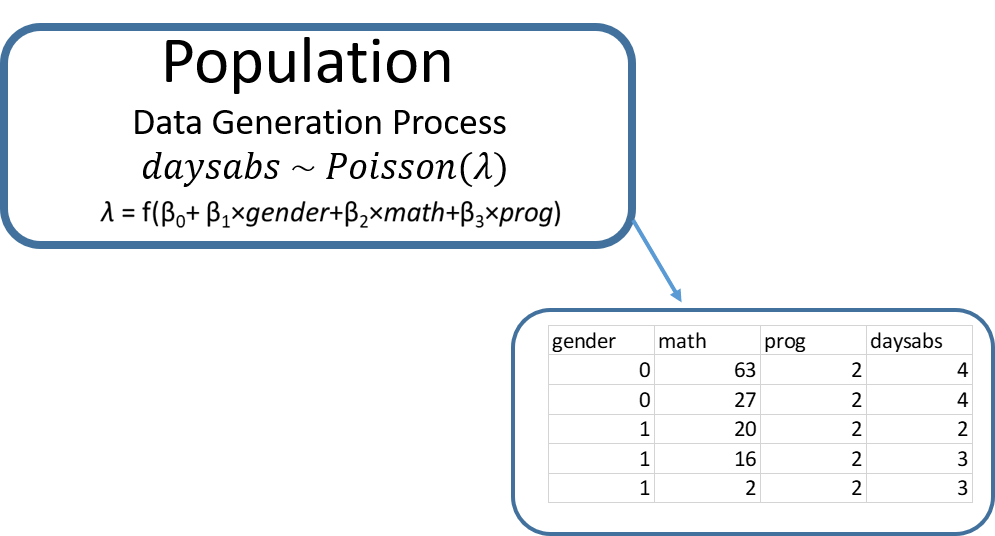
\includegraphics{estpic14.png}

As the domain of \(\lambda\) is \((0,\infty)\) the link function is
specified as \(\lambda = e^X\). The following estimates the Poisson
regression.

\begin{Shaded}
\begin{Highlighting}[]
\NormalTok{LLpois }\OtherTok{=} \ControlFlowTok{function}\NormalTok{(b0, b1, b2, b3)\{}
\NormalTok{  X }\OtherTok{=}\NormalTok{ b0 }\SpecialCharTok{+}\NormalTok{ b1}\SpecialCharTok{*}\NormalTok{student}\SpecialCharTok{$}\NormalTok{gender }\SpecialCharTok{+}\NormalTok{ b2}\SpecialCharTok{*}\NormalTok{student}\SpecialCharTok{$}\NormalTok{math }\SpecialCharTok{+}\NormalTok{ b3}\SpecialCharTok{*}\NormalTok{student}\SpecialCharTok{$}\NormalTok{prog}
\NormalTok{  lam }\OtherTok{=} \FunctionTok{exp}\NormalTok{(X)}
\NormalTok{  p }\OtherTok{=} \FunctionTok{dpois}\NormalTok{(}\AttributeTok{x =}\NormalTok{ student}\SpecialCharTok{$}\NormalTok{daysabs, }\AttributeTok{lambda =}\NormalTok{ lam)}
\NormalTok{  LL }\OtherTok{=} \FunctionTok{sum}\NormalTok{(}\FunctionTok{log}\NormalTok{(p))}
  \FunctionTok{return}\NormalTok{(}\SpecialCharTok{{-}}\DecValTok{1}\SpecialCharTok{*}\NormalTok{LL)}
\NormalTok{\}}

\NormalTok{res5 }\OtherTok{=} \FunctionTok{mle2}\NormalTok{(}\AttributeTok{minuslogl =}\NormalTok{ LLpois, }\AttributeTok{start =} \FunctionTok{list}\NormalTok{(}\AttributeTok{b0 =} \FunctionTok{log}\NormalTok{(}\FloatTok{5.96}\NormalTok{), }\AttributeTok{b1 =} \DecValTok{0}\NormalTok{, }\AttributeTok{b2 =} \DecValTok{0}\NormalTok{, }\AttributeTok{b3 =} \DecValTok{0}\NormalTok{))}
\FunctionTok{summary}\NormalTok{(res5)}
\end{Highlighting}
\end{Shaded}

\begin{verbatim}
## Maximum likelihood estimation
## 
## Call:
## mle2(minuslogl = LLpois, start = list(b0 = log(5.96), b1 = 0, 
##     b2 = 0, b3 = 0))
## 
## Coefficients:
##     Estimate Std. Error z value                Pr(z)    
## b0  3.255504   0.081341   40.02 < 0.0000000000000002 ***
## b1  0.235355   0.046742    5.04           0.00000048 ***
## b2 -0.007665   0.000923   -8.30 < 0.0000000000000002 ***
## b3 -0.606762   0.036192  -16.77 < 0.0000000000000002 ***
## ---
## Signif. codes:  0 '***' 0.001 '**' 0.01 '*' 0.05 '.' 0.1 ' ' 1
## 
## -2 log L: 2649
\end{verbatim}

The Poisson regression equation is

\[ln(\lambda) = 3.26 + 0.24 \times gender -0.0077 \times math -0.607 \times prog\]

All variables are statistically significant. Let us understand the
marginal effects. The coefficient for gender is 0.24. Gender is coded as
0 for females and 1 for males. \[ln(\lambda_1) - log(\lambda) = 0.24\]

With some alegbra we get,

\[\lambda_1 = e^{0.24} \lambda\]

and thus

\[\lambda_1 = 1.27\lambda\]

This means that the average number of days a male student is absent is
1.27 times that of a female student.

\hypertarget{model-fit}{%
\section{Model Fit}\label{model-fit}}

With linear regression \(R^2\) is used as a measure of the models
performance. The same concept does not translate to binary and count
models.

For a binary regression, a few metrics are useful to assess the model
fit. The first is the likelihood, which is normally reported as -2LL.
Note that we want this to be smaller. For the baseline model the value
of -2LL was 499.9765. For the logistic regression, it is 459.8384.
Hence, the regression model is better than the baseline model. Two other
metrics that are commonly used are AIC (Akaike Information Criteria) and
BIC (Bayesian Information Criteria). There are defined as:
\[𝐴𝐼𝐶 = −2𝐿𝐿 + 2𝑘\] \[𝐵𝐼𝐶 = −2𝐿𝐿 + 2𝑘𝑙𝑜𝑔(𝑛)\] Where \(k\) is the number
of parameters to be estimated and \(n\) is the number of observations.

Let us compute these for the Poisson model.

\begin{longtable}[]{@{}lll@{}}
\toprule()
Metric & Baseline Model & Poisson Regression \\
\midrule()
\endhead
\(-2LL\) & 3101.018 & 2648.787 \\
\(AIC\) & 3103.018 (k = 1) & 2656.787 (k = 4) \\
\(BIC\) & 3112.517 & 2694.782 \\
\bottomrule()
\end{longtable}

\begin{center}\rule{0.5\linewidth}{0.5pt}\end{center}

The metrics clearly indicate that the Poisson regression model is adding
value over the baseline model.

\hypertarget{glm-function}{%
\section{glm() function}\label{glm-function}}

The function to estimate a regression model with binary or count
outcomes in R is \texttt{glm()}. The general syntax is:

\texttt{glm(formula,\ family=familytype(link=linkfunction),\ data=)}

\begin{longtable}[]{@{}ll@{}}
\toprule()
Family & Default Link Function \\
\midrule()
\endhead
binomial & (link = ``logit'') \\
gaussian & (link = ``identity'') \\
Gamma & (link = ``inverse'') \\
inverse.gaussian & (link = ``1/mu\^{}2'') \\
poisson & (link = ``log'') \\
quasi & (link = ``identity'', variance = ``constant'') \\
quasibinomial & (link = ``logit'') \\
quasipoisson & (link = ``log'') \\
\bottomrule()
\end{longtable}

\begin{center}\rule{0.5\linewidth}{0.5pt}\end{center}

The following code estimates the binary and count models with our data.

\begin{Shaded}
\begin{Highlighting}[]
\NormalTok{res6 }\OtherTok{=} \FunctionTok{glm}\NormalTok{(admit}\SpecialCharTok{\textasciitilde{}}\NormalTok{gre}\SpecialCharTok{+}\NormalTok{gpa}\SpecialCharTok{+}\NormalTok{rank,}\AttributeTok{family=}\StringTok{"binomial"}\NormalTok{,}\AttributeTok{data=}\NormalTok{admit)}
\FunctionTok{summary}\NormalTok{(res6)}
\end{Highlighting}
\end{Shaded}

\begin{verbatim}
## 
## Call:
## glm(formula = admit ~ gre + gpa + rank, family = "binomial", 
##     data = admit)
## 
## Deviance Residuals: 
##    Min      1Q  Median      3Q     Max  
## -1.580  -0.885  -0.638   1.157   2.173  
## 
## Coefficients:
##             Estimate Std. Error z value Pr(>|z|)    
## (Intercept) -3.44955    1.13285   -3.05   0.0023 ** 
## gre          0.00229    0.00109    2.10   0.0356 *  
## gpa          0.77701    0.32748    2.37   0.0177 *  
## rank        -0.56003    0.12714   -4.40 0.000011 ***
## ---
## Signif. codes:  0 '***' 0.001 '**' 0.01 '*' 0.05 '.' 0.1 ' ' 1
## 
## (Dispersion parameter for binomial family taken to be 1)
## 
##     Null deviance: 499.98  on 399  degrees of freedom
## Residual deviance: 459.44  on 396  degrees of freedom
## AIC: 467.4
## 
## Number of Fisher Scoring iterations: 4
\end{verbatim}

\begin{Shaded}
\begin{Highlighting}[]
\NormalTok{res7 }\OtherTok{=} \FunctionTok{glm}\NormalTok{(daysabs}\SpecialCharTok{\textasciitilde{}}\NormalTok{gender}\SpecialCharTok{+}\NormalTok{math}\SpecialCharTok{+}\NormalTok{prog,}\AttributeTok{family=}\StringTok{"poisson"}\NormalTok{,}\AttributeTok{data=}\NormalTok{student)}
\FunctionTok{summary}\NormalTok{(res7)}
\end{Highlighting}
\end{Shaded}

\begin{verbatim}
## 
## Call:
## glm(formula = daysabs ~ gender + math + prog, family = "poisson", 
##     data = student)
## 
## Deviance Residuals: 
##    Min      1Q  Median      3Q     Max  
## -4.073  -2.268  -0.970   0.781   7.292  
## 
## Coefficients:
##              Estimate Std. Error z value             Pr(>|z|)    
## (Intercept)  3.254816   0.081352   40.01 < 0.0000000000000002 ***
## gender       0.235542   0.046747    5.04           0.00000047 ***
## math        -0.007633   0.000923   -8.27 < 0.0000000000000002 ***
## prog        -0.607277   0.036192  -16.78 < 0.0000000000000002 ***
## ---
## Signif. codes:  0 '***' 0.001 '**' 0.01 '*' 0.05 '.' 0.1 ' ' 1
## 
## (Dispersion parameter for poisson family taken to be 1)
## 
##     Null deviance: 2217.7  on 313  degrees of freedom
## Residual deviance: 1765.5  on 310  degrees of freedom
## AIC: 2657
## 
## Number of Fisher Scoring iterations: 5
\end{verbatim}

\end{document}
